% Copyright 2007 by Till Tantau
%
% This file may be distributed and/or modified
%
% 1. under the LaTeX Project Public License and/or
% 2. under the GNU Public License.
%
% See the file doc/licenses/LICENSE for more details.


\lecture[20]{Analysis of Variance}{lecture-text}

\subtitle{or, ANOVA}

\date{14 April 2015}

% pp 414-427

\begin{document}

\begin{frame}
  \maketitle
\end{frame}


\begin{frame}\frametitle<presentation>{Outline}
  \tableofcontents
\end{frame}

\section{Chi-squared recap}

\begin{frame}{Recap of chi-squared}
  \begin{block}{The $\chi^2$ test for an $r \times k$ table:}
    $H_0:$ The row and column variables are \alert{independent}, i.e.\\
      the population distribution of row categories is the same for each column 
      as for the entire population.\\
    $H_A:$ The population distributions of some columns differ from others. \\


    \alert{Test statistic:}
    \begin{align*}
      \chi^2_s &= \sum_{i,j} \frac{ (\text{observed}_{i,j} - \text{expected}_{i,j})^2 }{ \text{expected}_{i,j} }  \\
      \text{expected}_{ij} &= \frac{ \text{(row $i$ total)} \times \text{(column $j$ total)} }{ \text{(grand total)} } \\
      \df &= (r-1)(k-1)
    \end{align*}


    \alert{Conditions:} 
    \begin{itemize}
      \item Independent samples, either within columns, or in total.
      \item Sample size: each expected count ${}\ge 5$.
      \item Conclusion is ``omnidirectional''.
    \end{itemize}

  \end{block}
\end{frame}

\begin{frame}{Example: hair and eye color}

  of 6,800 independent, randomly sampled, German men.
  \begin{center}
    \begin{tabular}{ll|rrrr}
      & & & \multicolumn{2}{c}{hair color} & \\
      & & brown & black & fair & red \\
      \hline
      & brown & 438 & 288 & 115 & 16 \\
      eye color & grey/green & 1387 & 746 & 946 & 53 \\
      & blue & 807 & 189 & 1768 & 47 \\
    \end{tabular}
  \end{center}

    \vspace{2em}
    \pause

    $H_0$: Hair and eye color are \alert{independent}. \\
    $H_A$: Hair and eye color are \alert{not} independent. 

    \vspace{2em}
    \pause

  \begin{center}
    \only<3>{
    \begin{tabular}{ll|rrrr|r}
      \alert{hair | eye} & & & \multicolumn{2}{c}{hair color} & & \\
      & & brown & black & fair & red & mean \\
      \hline
                 & brown  & 0.17 & 0.24 & 0.04 & 0.14 & 0.15 \\ 
  eye color & grey/green  & 0.53 & 0.61 & 0.33 & 0.46 & 0.48 \\ 
                  & blue  & 0.31 & 0.15 & 0.62 & 0.41 & 0.37 \\ 
                  \hline
                  & total & 1.0 &  1.0  & 1.0  & 1.0  & 
    \end{tabular}
    }\only<4>{
    \begin{tabular}{ll|rrrr|r}
      \alert{eye | hair} & & & \multicolumn{2}{c}{hair color} & \\
      & & brown & black & fair & red  & total \\
      \hline
               & brown   & 0.51 & 0.34 & 0.13 & 0.02  & 1.0 \\ 
eye color & grey/green   & 0.44 & 0.24 & 0.30 & 0.02  & 1.0 \\ 
                & blue   & 0.29 & 0.07 & 0.63 & 0.02  & 1.0 \\ 
                \hline
                & mean &  0.41  & 0.21 & 0.36 & 0.01  & 
    \end{tabular}
    }
  \end{center}


\end{frame}

\begin{frame}{Example: hair and eye color}

  \begin{center}
    \begin{tabular}{ll|rrrr|r}
  \alert{Observed:} & & & \multicolumn{2}{c}{hair color} & \\
      & & brown & black & fair & red  & total\\
      \hline
      & brown & 438 & 288 & 115 & 16 & 857 \\
      eye color & grey/green & 1387 & 746 & 946 & 53 & 3132 \\
      & blue & 807 & 189 & 1768 & 47 & 2811 \\
      \hline 
      & & 2632 & 1223 & 2829  & 116  & 6800 \\
    \end{tabular}
  \end{center}
  % x <- c(438, 1387, 807, 288, 746, 189, 115, 946, 1768, 16, 53, 47)
  % dim(x) <- c(3,4)

  \begin{center}
    \begin{tabular}{ll|rrrr|r}
  \alert{Expected:} & & & \multicolumn{2}{c}{hair color} & \\
      & & brown & black & fair & red  & total\\
      \hline
                 & brown  & 331.71 & 154.13 & 356.54 & 14.62   & 857  \\ 
  eye color & grey/green  & 1212.27 & 563.30 & 1303.00 & 53.43 & 3132 \\ 
                  & blue  & 1088.02 & 505.57 & 1169.46 & 47.95 & 2811 \\ 
      \hline 
      & & 2632 & 1223 & 2829  & 116  & 6800 \\
    \end{tabular}
  \end{center}
  % x <- c(438, 1387, 807, 288, 746, 189, 115, 946, 1768, 16, 53, 47)
  % dim(x) <- c(3,4)

  \begin{center}
    \begin{tabular}{ll|rrrr|r}
  \alert{Difference:} & & & \multicolumn{2}{c}{hair color} & \\
      & & brown & black & fair & red  & total\\
      \hline
                 & brown  & 106.29 & 133.87 & -241.54 & 1.38    & 0  \\ 
  eye color & grey/green  & 174.73 & 182.70 & -357.00 & -0.43   & 0 \\ 
                  & blue  & -281.02 & -316.57 & 598.54 & -0.95  & 0 \\ 
      \hline 
      & & 0 & 0 & 0  & 0 & 0 \\
    \end{tabular}
  \end{center}
  % x <- c(438, 1387, 807, 288, 746, 189, 115, 946, 1768, 16, 53, 47)
  % dim(x) <- c(3,4)

  \begin{align*}
  \end{align*}

\end{frame}

\begin{frame}{Example: hair and eye color}

  \begin{align*}
    \chi^2_s &= \frac{106.29^2}{331.71} + \frac{133.87^2}{154.13} + \cdots + \frac{(-0.95)^2}{47.95} \\
        &= 1073.508
  \end{align*}
  With $\df = (3-1)\times(4-1) = 6$, \\
  since $\chi^2_{6,0.0001} = 27.86$, 
  $P \ll 0.0001$.

  \vspace{2em}

  We have \alert{very strong} evidence that hair and eye color are \alert{not} independent.


\end{frame}


\section{Multiple groups}

\begin{frame}{Moving on\ldots}
  \begin{enumerate}
    \item Recall the $t$-test:
    \item that let us \alert{compare the means} of two independent samples:
      \begin{center}
        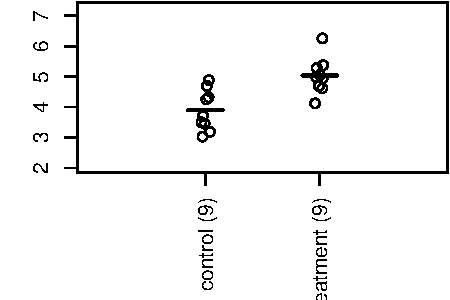
\includegraphics{dots1ex}
      \end{center}
    \item What about more categories?
    \item more complicated combinations?
  \end{enumerate}
\end{frame}

\begin{frame}{Example}

  Beak length for 32 birds of the same species on three islands that differ in ecology:
\begin{center}
  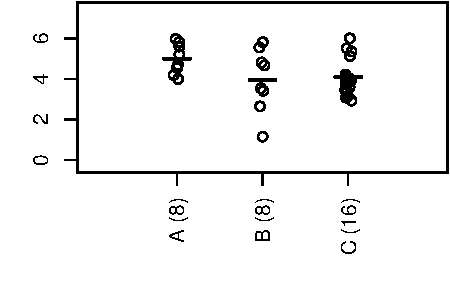
\includegraphics{dots2ex.pdf}
\end{center}

    \vspace{1em}

    \structure{Question:} Is there a significant difference in mean beak length between the islands?

    \vspace{2em}

    \structure{$H_0$:} All the means are the same.
    ($\mu_A = \mu_B = \mu_C$)

\end{frame}

%%%%%%
\begin{frame}{Why not use paired tests?}

  We could compare $A$ to $B$, $A$ to $C$, and $B$ to $C$.\\
  \structure{But:}
  \begin{itemize}
    \item \alert{multiple testing} makes things difficult
    \item since at $\alpha=.05$, one in twenty true null hypotheses will be rejected
    \item and the tests aren't independent of each other.
  \end{itemize}

    \vspace{2em}

    A single framework (\alert{one-way ANOVA}) is more elegant,\\
    and lets us \alert{pool information} across all samples.

\end{frame}

% MORE ON MULTIPLE TESTING?

%%%%%%
\begin{frame}{ANalysis Of VAriance}

  ANOVA compares
  \begin{itemize}
    \item variance \alert<1>{within} groups 
    \item to the variance \alert<2>{between} groups 
  \end{itemize}

    \vspace{2em}

  \begin{center}
    \includegraphics<1>{dots2ex-within.pdf}
    \includegraphics<2->{dots2ex-between.pdf}
  \end{center}


\end{frame}

\section{One-way ANOVA:}

\begin{frame}{Notation}

  \begin{itemize}
    \item[$y_{ij}$:] the $j^\mathrm{th}$ observation in group $i$
    \item[$I$:] number of groups
    \item[$n_i$:] number of obs. in $i^\mathrm{th}$ group
    \item[$\bar y_i$:] (sample) mean of the $i^\mathrm{th}$ group
    \item[$s_i$:] (sample) SD for the $i^\mathrm{th}$ group
  \end{itemize}

  and

  \begin{itemize}
    \item[$n_\cdot$:] total number of observations
    \item[$\bar {\bar y}$:] grand mean of the observations
  \end{itemize}

  where

  \begin{align*}
    {\bar y}_i &= \frac{1}{n_i}\sum_{j} y_{ij} \\
    \bar {\bar y} &= \frac{1}{n_\cdot}\sum_{ij} y_{ij} \\
  \end{align*}

\end{frame}

%%%%%%
\begin{frame}{Within-group variation}

  Recall that the \structure{sample variance} is \\
  the sum of the squared deviation from the sample average,\\
  divided by the degrees of freedom:
  \[
  s_i^2 = \frac{ \sum_j (y_{ij}-\bar y_i)^2 }{ n_i-1 } = \frac{ (y_{i1} - \bar y_i)^2 + \cdots + (y_{in_i} - \bar y_i)^2 }{n_i-1}
  \]

    \vspace{2em}

    The ``\alert{Mean Square Within Groups}'' is analogous, across all groups:
    \begin{align*}
      \SS(\text{within}) &= \sum_{i} (n_i-1) s_i^2 = \sum_{ij} (y_{ij}-\bar y_i)^2 \\
      \df(\text{within}) &= n_\cdot - I \\
      \MS(\text{within}) &= \frac{\SS(\text{within})}{\df(\text{within})}
    \end{align*}

    Another name for $\MS(\text{within})$ is the ``pooled variance''.

\end{frame}

%%%%%%
\begin{frame}{Between-group variation}

  What's left over? 
  Think of the ``\alert{Mean Square Between Groups}'' 
  as the variance, after replacing all observations by their group mean:
  \begin{align*}
    \SS(\text{between}) &= \sum_{i} n_i (\bar y_i - \bar{\bar y}_i)^2 \\
      \df(\text{between}) &= I - 1 \\
      \MS(\text{between}) &= \frac{\SS(\text{between})}{\df(\text{between})}
  \end{align*}

\end{frame}

%%%%%%
\begin{frame}{Within versus Between}

  Think of it as taking variances of these terms separately:
  \[ y_{ij} = \bar y_i + (y_{ij} - \bar y_i) \]

    \vspace{2em}


  \begin{center}
    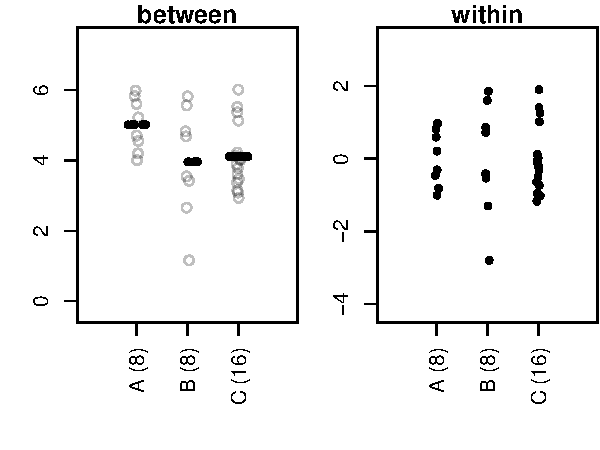
\includegraphics[width=\textwidth]{dots2ex-within-between.pdf}
  \end{center}

\end{frame}

%%%%%%
\begin{frame}{Total Sum of Squares}

  The \alert{total sum of squares} is
  \[ \SS(\text{total}) = \sum_{ij} (y_{ij} - \bar{\bar y})^2 , \]
  or the sum of squared deviations from the grand mean.

    \vspace{2em}

  \structure{Remarkably,} the ``between'' and ``within'' sum of squares \\
  \alert{exactly partition} the total sum of squares:
  \[  \SS(\text{total})  = \SS(\text{between}) + \SS(\text{within}) \]
  \ldots thanks, Pythagoras.

    \vspace{2em}

    The associated degrees of freedom is also partitioned:
    \[ \df(\text{total}) = n_\cdot - 1 = \df(\text{between}) + \df(\text{within}) .  \]


\end{frame}

\section{The ANOVA table}


%%%%%%
\begin{frame}{Displaying and ANOVA}

  To summarize:
  \begin{center}
    \begin{tabular}{lrrr}
      source & df & SS & MS \\
      \hline
      between groups & $I-1$ & $\sum_i n_i (\bar y_i - \bar{\bar y})^2$  & $\SS/\df$ \\
      within groups & $n_\cdot -I$ & $\sum_i (n_i -1 )s_i^2$ & $\SS/\df$ \\
      \hline
      Total & $n_\cdot -1$  & $\sum_{ij} (y_{ij}-\bar{\bar y})^2$  & \\
    \end{tabular}
  \end{center}


\end{frame}


\section{Examples}


%%%%%%
\begin{frame}{Example I}

\begin{tabular}{ll|rr}
  value & group & $\bar y_i$ & $y_{ij}-\bar y_i$  \\ 
  \hline
3   &  A  &  5.75  &  -2.75      \\
7   &  A  &  5.75  &  1.25       \\
8   &  A  &  5.75  &  2.25       \\
5   &  A  &  5.75  &  -0.75      \\
6   &  B  &  5.00     &  1.00          \\
5   &  B  &  5.00     &  0.00          \\
5   &  B  &  5.00     &  0.00          \\
10  &  B  &  5.00     &  5.00          \\
2   &  B  &  5.00     &  -3.00         \\
3   &  B  &  5.00     &  -2.00         \\
2   &  B  &  5.00     &  -3.00         \\
7   &  B  &  5.00     &  2.00        \\
   \hline
   & SS & 1.5 & 66.75 \\ 
   & df & 1 & 10 \\ 
   & MS & 0.15 & 6.675   \\ 
\end{tabular}

\end{frame}

%%%%%%
\begin{frame}{Summarized, ANOVA-style}

  \begin{center}
    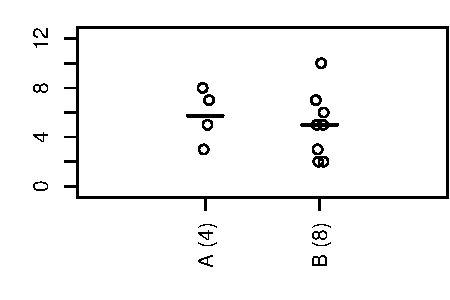
\includegraphics{dots3ex.pdf}

    \vspace{2em}

    \begin{tabular}{lrrr}
      source & df & SS & MS \\
      \hline
      between groups & 1 & 1.5 & 1.5 \\
      within groups & 10 & 66.75 & 6.675 \\
      \hline
      Total & 11 & 68.25 & \\
    \end{tabular}

  \end{center}

\end{frame}

%%%%%%
\begin{frame}{Example 2:}

\begin{tabular}{ll|ll}
  \hline
  value & group & $\bar y_i$ & $y_{ij} - \bar y_i$ \\ 
  \hline
12  &   A  &       11.5  &       0.5      \\
15  &   A  &       11.5  &       3.5      \\
9   &   A  &       11.5  &       -2.5     \\
10  &   A  &       11.5  &       -1.5     \\
2   &   B  &       4.25  &       -2.25    \\
7   &   B  &       4.25  &       2.75     \\
4   &   B  &       4.25  &       -0.25    \\
1   &   B  &       4.25  &       -3.25    \\
9   &   B  &       4.25  &       4.75     \\
2   &   B  &       4.25  &       -2.25    \\
2   &   B  &       4.25  &       -2.25    \\
7   &   B  &       4.25  &       2.75     \\
   \hline
&   SS  &  140.1667  &     84.5  \\
&   df  &  1       &     10      \\
&   MS  &  140.1667  &     8.45   \\
\end{tabular}
\end{frame}

%%%%%%
\begin{frame}{Summarized, ANOVA-style}

  \begin{center}
    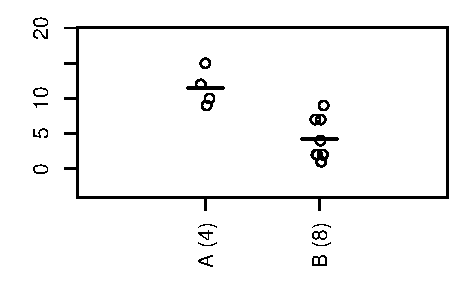
\includegraphics{dots4ex.pdf}

    \vspace{2em}

    \begin{tabular}{lrrr}
      source & df & SS & MS \\
      \hline
      between groups & 1 & 140.1667 & 140.1667 \\
      within groups & 10 & 84.5 & 8.45 \\
      \hline
      Total & 11 & 224.6667 &  \\
    \end{tabular}

  \end{center}

\end{frame}

%%%%%%
\begin{frame}{Thinking about it}

  With fixed sample sizes, what does it mean if
  \begin{enumerate}
    \item $\SS(\text{within})$ is small?
    \item $\SS(\text{between})$ is small?
    \item $\SS(\text{within})$ is small relative to $\SS(\text{between})$?
    \item $\MS(\text{within})$ is small relative to $\MS(\text{between})$?
  \end{enumerate}

\end{frame}

\section<article>{Summary}
\section<presentation>*{Summary}

\begin{frame}{Summary}
  \begin{enumerate}
    \item Goal: compare means between many groups of independent observations.
    \item Tool: \alert{analysis of variance}, or ANOVA
    \item that partitions the ``total variance'' into two pieces, roughly:
    \item variance of group means (``between''), and
    \item variance of deviations from group means (``within'').
  \end{enumerate}
  Next time: a test statistic and a distribution.
\end{frame}

% homework
\begin{frame}{Homework}
  \begin{center}

  11.2.1

  \vspace{2em}

  11.2.7

  \vspace{2em}

  % 7.5.1

  \end{center}
\end{frame}


\end{document}





